\documentclass[../syllabus.tex]{subfiles}

\begin{document}

\section{Leerdoelen}
\begin{itemize}
    \item Begrip voor het concept recursie
    \item Het coderen van recursieve functies
    \item Het kunnen tekenen van simple fractels
\end{itemize}

\section{Uitleg}
\begin{itemize}
    \item \myhref{https://www.youtube.com/watch?v=-wiverLQl1Q\&list=PLRqwX-V7Uu6bXUJvjnMWGU5SmjhI-OXef\&index=1}{Fractals - The Nature of Code}\\
    Alleen \textbf{8.1, 8.2, 8.3}\\
    \textit{Bij 8.3 wordt er gebruik gemaakt van een \texttt{ArrayList} voor het maken van Koch's Curve. Dit hoef je (nog) niet te kunnen.}
    \item \myhref{https://natureofcode.com/book/chapter-8-fractals/}{Chapter 8. Fractals}\\
    Alleen \textbf{8.1, 8.2, 8.3, 8.4, 8.5}\\
    \textit{Bij 8.4 wordt er gebruik gemaakt van een \texttt{ArrayList} voor het maken van Koch's Curve. Dit hoef je (nog) niet te kunnen.}
\end{itemize}

\newpage
\section{Opdrachten}
\subsection{[Optioneel] Recursieve functies}
Recursieve functies zijn functies die een (makkelijkere) versie van zichzelf gebruiken voor het bereken van een antwoord. Kijk bijvoorbeeld naar:
\[f(n) = \begin{cases}
        $1 \qquad\qquad\qquad n = 0$\\
        $3 * f(n-1)  \qquad n $>$ 0$
    \end{cases}
   \]
Deze functie geeft $f(n) = g^n$. Als we dit uitschrijven krijgen we: $f(4) = 3 * f(3) = 3 * 3 * f(2) = 3 * 3 * 3 * f(1) = 3 * 3 * 3 * 3 * f(0) = 3 * 3 * 3 * 3 * 1 = 81 = 3^4$
\[g(n) = \begin{cases}
        $1 \qquad\qquad\qquad n = 0$\\
        $n * g(n-1)  \qquad n $>$ 0$
    \end{cases}
   \]
Schrijf de uitwerking van $g(5)$ helemaal uit. Weet je ook welke functie $g$ is?
\[h(n) = \begin{cases}
        $1 \qquad\qquad\qquad n = 0$\\
        $1 \qquad\qquad\qquad n = 1$\\
        $h(n - 1) + h(n - 2)  \qquad n $>$ 1$
    \end{cases}
   \]
Schrijf de uitwerking van $h(4)$ helemaal uit. Weet je ook welke functie $h$ is?

\subsection{Recursieve circles}
Als een functie \textit{zichzelf} aanroept noemen we dit \textbf{recursie}. 
Je kunt met recursie allerlei coole dingen tekenen. Een recursieve functie moet wel ooit stoppen, daarom geeft je vaak een getal mee \texttt{int n} wat het aantal \textbf{itteraties} geeft, ofwel, hoe vaak de functie aangeroepen wordt, of hoe "diep" de functie gaat.\\
Pas de onderstaande code aan zodat het resultaat lijkt op figuur \ref{fig:recursive_circles}
\begin{lstlisting}
void recursiveCircles(int n, PVector pos) {
  if (n > 0) { 
    circle(pos.x,pos.y,n * 10);
    recursiveCircles(n - 1,pos);
  }
}
\end{lstlisting}
\begin{figure}[H]
	\centering
	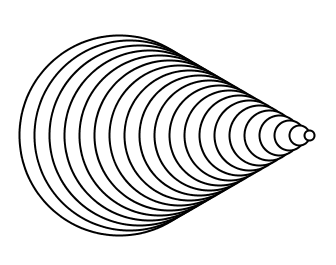
\includegraphics[width=4cm]{recursive_circles.png}
	\caption{Recursief getekende cirkels}
	\label{fig:recursive_circles}
\end{figure}

\subsection{Maak een binary tree}
In deze opdracht ga je een \textbf{binary tree} maken (zie figuur \ref{fig:binary_tree}). Een binary tree bestaat uit \'e\'en lijn, genaamd de stam (trunk). Vanuit de top van deze stam "groeien" weer twee nieuwe stammen, alleen dan gedraaid onder een hoek. Maak de functie \texttt{binaryTree} af.
\begin{lstlisting}
void binaryTree(int n,PVector pos,PVector trunk) {
  if (n > 0) {
    PVector tip = pos.copy().add(trunk);
    line(pos.x,pos.y,tip.x,tip.y);
  }
}
\end{lstlisting}
\begin{figure}[H]
	\centering
	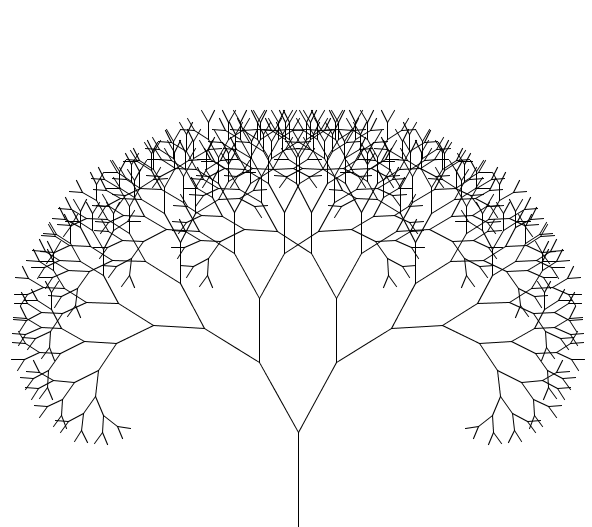
\includegraphics[width=8cm]{binary_tree.png}
	\caption{Een binary tree}
	\label{fig:binary_tree}
\end{figure}

\subsection{Meer soorten trees!}
Vervang de hoek die je gebruikt hebt bij de vorige opdracht door \texttt{(float) mouseX / width)}. Aanschouw de epische trees!
\remark{Zorg ervoor dat je de functie aanroept in de \texttt{draw} functie}

\end{document}